\documentclass{beamer}
\usetheme{Frankfurt}
\usecolortheme{seahorse}
\title{Parsing Expression Grammars}
\author{Niccolò Piazzesi}
\institute[UniPi]{
    Università degli Studi di Pisa \\
    Anno Accademico 2020-21
}
\beamertemplatenavigationsymbolsempty
\setbeamertemplate{footline}[page number]
\AtBeginSection[]{
  \begin{frame}
  \vfill
  \centering
  \begin{beamercolorbox}[sep=8pt,center,shadow=true,rounded=true]{title}
    \usebeamerfont{title}\insertsectionhead\par%
  \end{beamercolorbox}
  \vfill
  \end{frame}
}

\begin{document}
    \begin{frame}
        \maketitle
    \end{frame}
    \section{Parsing}
    \begin{frame}
        \begin{block}{What's a parser?}
            Part of the compiler.
            Checks the stream of tokens produced by the \emph{lexer} for syntactical errors
            and produces an IR representation (usually an abstract syntax tree) of the source 
            that is used in later steps to generate machine code.
        \end{block}
        \begin{figure}
            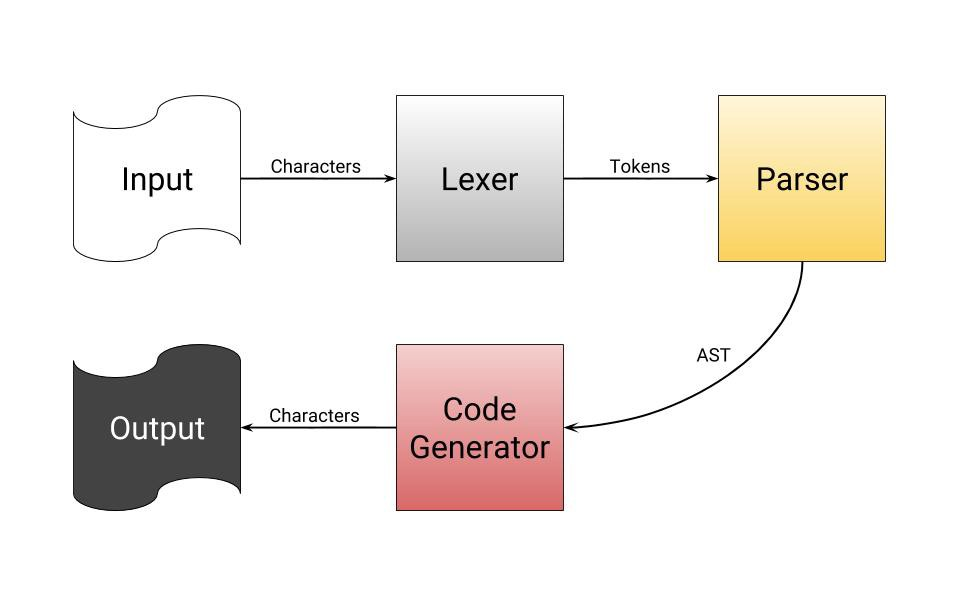
\includegraphics[width=\textwidth]{img/parser.jpg}
        \end{figure}
    \end{frame}
    \begin{frame}
        \frametitle{Context free grammars}
        \begin{block}{}A programming language syntax can be described using a context free grammar G.\end{block}

        \begin{block}{}We want to check if the source code is actually valid code\end{block}
    \end{frame}
    \begin{frame}
        Given the rules of grammar G, we want to find a sequence of rule applications that generates a target expression (\textbf{derivation}).

        Parsing is the process of discovering such sequence.
    \end{frame}
    \section{Formal definiton of PEG}
    \section{A concrete example: \emph{pgen}}
\end{document}